\documentclass[12pt]{report}
\usepackage[utf8]{inputenc}
\usepackage{graphicx}
\graphicspath{{images/}}
\usepackage[a4paper,width=150mm,top=25mm,bottom=25mm]{geometry}
\usepackage{fancyhdr}
\pagestyle{fancy}
\fancyhead{}
% \fancyhead[LO,LE]{Chapter \thechapter}
\fancyhead[LO]{\leftmark}
\fancyfoot{}
\fancyfoot[CO]{\thepage}
\usepackage{indentfirst}
\usepackage{tocbibind}

% use style=superborder to create table
\usepackage[acronym,nomain,nopostdot,nogroupskip,style=super,nonumberlist,toc]{glossaries}
% Generate the glossary
\makeglossaries


\title{
    {\huge Ho Chi Minh City University of Technology}\\
    {
\includegraphics[width=100mm, scale=0.7]{BK_logo.png}}\\
    {\huge Smart Home}\\
}
\author{Student: Tuan-Hung VU\\ID: 1450231}
\date{Day Month Year}

%include glossaries files
% %Term definitions
% \newglossaryentry{alu}{name=ALU, description={Arithmetic Logic Unit}}
% \newglossaryentry{mcu}{name=MCU, description={Microcontroller Unit}}
% \newglossaryentry{cu}{name=CU, description={Control Unit}}
\newacronym{alu}{ALU}{Arithmetic Logic Unit}
\newacronym{adc}{ADC}{Analog to Digital Converter}
\newacronym{dac}{DAC}{Digital to Analog Converter}
\newacronym{mcu}{MCU}{Microcontroller Unit}
\newacronym{cu}{CU}{Control Unit}
\newacronym{ram}{RAM}{Random Access Memory}
\newacronym{rom}{ROM}{Read-only Memory}
\newacronym{cpu}{CPU}{Central Processing Unit}
\newacronym{mqtt}{MQTT}{Message Queue Telemetry Transport}


%------------------------------------------------------------
\begin{document}
%make title works
\maketitle
%------------------------------------------------------------
\pagenumbering{roman}
\chapter*{Abstract}
Nowadays, an Automation Home is not a new definition for people, especially with the evolution of the technology. In comparison to the old days, in which people were not even think about controlling light in a far distance without touching the button, but things have changed, now people can do even more than that. In addition, controlling devices in a house now can be done in a very long distance with an easy click or probably a tap from a smart device like smartphone or personal computer. Furthermore, with the purpose of maximization the convenience for everyday life, scenarios are built to satisfy specified scenarios in everyday routine. Not to mention, with the raising of the trend to analyze collected data, people can develop even more features to serve people life.

This thesis is implemented with the basic features of an automation house such as controlling devices in decent distance in an effortless way, or the owner can control the devices in different rooms with physical or virtual switches. Last but not least, it is successfully built in with a Web Server to control devices from endless distance and a Security Camera block to open door automatically with Facial Recognition system. The Database is also integrated in every steps of the system in order to collect data for maintaining system and using for further development.


\chapter*{Acknowledgements}
I am profoundly grateful to Dr.Trinh Hoang Hon for his expert guidance and continuous encouragement throughout to see that this project rights its target since its commencement to its completion.

Again, I would like to express deepest appreciation towards Dr.Trinh Hoang Hon, whose invaluable guidance supported us in completing this project. He inspired me as similarly as equipped me with more knowledge about my major.

I also want to thank Mr. Truong Ha Giang, Mr. Nguyen Tai Hau, Mr. Le Duy Nguyen Bao who are my friends and helped me when I need help the most for this thesis.

At last I must express our sincere heartfelt gratitude to all the staff members of Electrical and Electronics Engineering faculty who helped me directly or indirectly during this course of work.

\begin{flushright}
    Ho Chi Minh City, December $24^{th}$, 2018\\
    Vu Tuan Hung.
\end{flushright}

\tableofcontents
% \listoffigures
% use below block to add "Figure" in front of aption in list of figures
{%
\let\oldnumberline\numberline%
\renewcommand{\numberline}{\figurename~\oldnumberline}%
\listoffigures%
}
% List of Tables
\listoftables
%Print the glossary
\printglossary[title={Acronym and Abbreviation}]
%-------------------------------------------------------------
\newpage
\setcounter{page}{1}
\pagenumbering{arabic}
% Main Chapters
\chapter{Introduction}
\section{Overview}
Smart Home is considered as a House with the integration of automation system, in which connects from one to another in order to control devices in an effortless way. To be specific, people can control specified device with physical button in any room and from any room. Not to mention, the system also helps people with controlling devices from distance without touching the physical buttons by using a Web Server User Interface on personal computer or a smart device. With the development speed of technology, the devices in a house, namely Television, conditioner, lights or camera can be connected with each other with or without a central device and work as programmed scenarios.
\begin{figure}[!ht]
    \begin{center}
    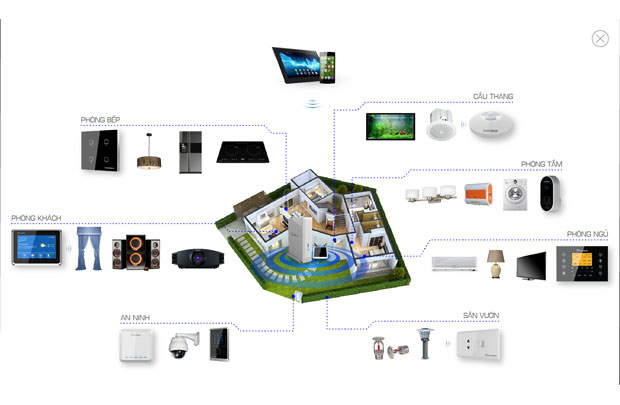
\includegraphics[scale=0.6]{images/overview.jpg}
    \caption{Overview of a Smart Home}
    \label{fig:overviewSmartHome}
    \end{center}
  \end{figure}

Besides, the house is usually implemented with sensors in order to collect environment data to maintain the best environment for the owner by controlling the devices such as conditioner, fan or curtains or to alert if a dangerous circumstance could happen.

\section{Current Research}
    With the rapidly growing of technology, especially connecting devices with the Internet becomes the trend today. Internet of Things is the combination of “things” including the new technology integrated thing or non-internet support thing but now is connected within the network, in order to connect and communicate to complete specified tasks.

    The connection between devices can be established via Wi-Fi, cellular network (3G, 4G and 5G in near future), Bluetooth, Zigbee or Infrared. The devices can be smartphones, circuit breakers, conditioner, headphones, light bulbs, and so on. The traditional devices (as they used to be) now can connect to the common network with a small integrated circuit with the function of establish any of connection mentioned above. However, letting a device running for 24 hours a day and 7 days a week is a real challenge because of their energy consumption, which is not solved effectively even in recent years.
    \subsection{Foreign Research}
    The giants in technology fields are already step into IoT field by providing services, software and hardware. For instance, Google introduced their Google Home with their voice recognition technology in order to automate the house activities. Beside Google, Amazon provides Amazon Echo and AWS with many integrated services which help their hardware products provided most satisfied experiences for the customers especially using Alex with trainable skill to control devices with voice recognition.

    In addition, there exists plenty of companies providing complete solution from hardware and extendable services to help with their products. For instance, Control4 is selling central device named EA series, focus on centralize control of devices and multimedia. Furthermore, their solution also included sensors integration in order to maintain the best environment for the users while using the house, such as dimming the light or pull curtains depends on day light insensitivity. 
    \subsection{Domestic Research}
    For domestic products, there are companies providing solutions based on foreign hardware in order to ensure the stability over time of the system. The company named Home Flow is an example who is providing the solutions and services based on Control4 and other foreign countries because Control4 products are opened source to ensure their partner can easily modify and extend their services. Moreover, there are companies that have strong potential of financial and research capability, namely Viettel or Bkav, they can research and introduce their own products. Thus, there is not yet remarkable products on the market by domestic companies.

\section{Thesis Objective}
In this thesis, the author only focus on implementing basic features for demonstration model with an advanced feature is Facial Recognition system embedded in a mini computer in order to run it without using a strong and costly personal computer, in which reduce the investment but still, achieve acceptable performance. The author will propose a centralize control model that can receive and distribute the command of controlling devices from distance by physical buttons in a flexible way and via Web Server with virtual buttons where user can control their devices from endless distance with the Internet Connection and a supported smart device. Last but not least, the thesis is also built in with a database in order to collect data for further development as data analysis is now becoming a serious trend along with the IoT applications.
\section{Thesis Structure}
This thesis consists of six chapters, in which are described as following.
\begin{itemize}
\item \textbf{Chapter 1}: Introduction of the project, which includes the idea of the author, project’s trend and some researches from foreign countries and also domestic ones.
\item \textbf{Chapter 2}: is the theory background of which the author read in order to collect appropriate knowledge to implement the project.
\item \textbf{Chapter 3}: is the hardware design, choosing components and sketch on Altium Designer with the overall hardware model.
\item \textbf{Chapter 4}: the software design for the system includes the algorithm of each implemented blocks.
\item \textbf{Chapter 5}: The results that the author achieved with real photos from the projects.
\item \textbf{Chapter 6}: Conclusion of the whole project with the limitations. In addition, the author also shows his future idea to improve the project.
\end{itemize}


 
\chapter{Background}
%for testing sectioning purpose
% \section{Test thu}
% \input{chapters/sections/sections2.1

\section{Microcontroller}
  \subsection{Theory}
  \gls{mcu} is a small size, special purpose computer. It is small enough in order to be integrated on a small circuit in which will do specified tasks or applications. MCU itself comes with memory, input, output peripherals and processor. Program to run the MCU is stored in \gls{rom} and usually not change in production. A microcontroller is usually designed to run in small size and at low cost, which is compatible to be embedded in other system in order to control actions of the system automatically.

  Few advantages of \gls{mcu} over a microprocessor can be listed as following:
  \begin{itemize}
    \item A MCU is already a standalone microcomputer.
    \item Because it can be considered as an independent computer, most needed components are integrated on a small size board.
    \item The above reason leads to the benefit that using MCU can make the system compact, highly mobile and cost efficiency.
    \item Time reduction because it is programed to run specified set of commands only.
    \item It is also easy to use and maintain.
    \item MCU nowadays usually designed to be used with low power in order to last longer under energy-limited condition.
  \end{itemize}

  \subsection{Microcontroller structure}
  Figure~\ref{fig:mcuStructure} demonstrates the basic structure of a microcontroller. It is easily to see the basic design of a microcontroller and its components.
  \begin{figure}[!ht]
    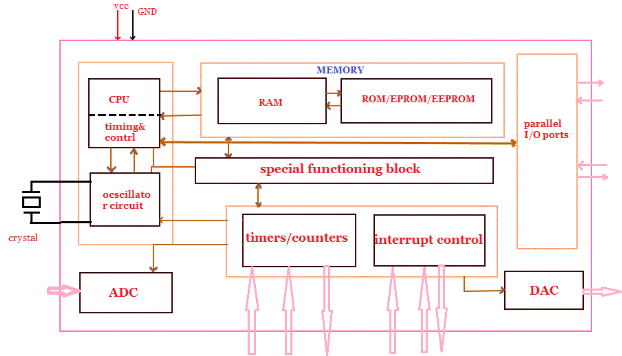
\includegraphics[scale=0.9]{images/Microcontroller-Structure.png}
    \caption{Structure of Microcontroller}
    \label{fig:mcuStructure}
  \end{figure}
  
  \begin{itemize}
    \item CPU: is the central unit which is assembled with \gls{alu} and a \gls{cu}. Its functions are connect parts of the MCU into a single system by doing fetch, decode and execution.
    \item Memory: there are two types of Memory that are required, namely \gls{rom} and \gls{ram}. Each type has its own functions, in which ROM will handle the program and the written instructions and RAM can only store temporary data while the program is executing.
    \item Input/Output: the single board system needs input to execute the program as well as outputs to delivery the information for further handling. The I/O peripherals are the interface of the MCU to communicate with or to control other devices.
    \item Bus: bus is the system of wires that used to connect the \gls{cpu} with other peripherals, which means it plays an important role but rarely discussed.
    \item Timers/Counters: they are built-in components for microcontroller, which is used to count in order to handle external events.
    \item Interrupts: is used to interrupt that can be an external or internal one, which helps to execute an instruction(s) while the main program is executing. 
    \item ADC: \gls{adc}, its name says it all, which is a circuit use to convert analogs signal to digital signals. The reason to use ADC is most sensors available on the market can read only analog signal but CPU of the \gls{mcu} can read digital signal only, so a \gls{adc} is necessary for them to communicate.
    \item DAC: \gls{dac} similar to \gls{adc}, DAC is also a circuit which convert digital signals into analog signals for further processing.
  \end{itemize}


  \subsection{Microcontroller market}
  There exists many microcontrollers on the market which come in various sizes and capacities. The list is only containing very few popular MCU that the author knows of.
  \begin{itemize}
    \item Intel 8051
    \item STMicroelectronics STM8S (8-bit), ST10 (16-bit) and STM32 (32-bit)
    \item Atmel AVR (8-bit), AVR32 (32-bit), and AT91SAM (32-bit)
    \item Freescale ColdFire (32-bit) and S08 (8-bit)
    \item PIC (8-bit PIC16, PIC18, 16-bit dsPIC33 / PIC24)
    \item Renesas Electronics: RL78 16-bit MCU; RX 32-bit MCU; SuperH; V850 32-
    bit MCU; H8; R8C 16-bit MCU
    \item PSoC (Programmable System-on-Chip)
    \item Texas Instruments Microcontrollers MSP430 (16-bit), C2000 (32-bit), and
    Stellaris (32-bit)
  \end{itemize}

\section{Communication}
  \subsection{Introduction}
  Nowadays, there are various communication protocols can be used for the thesis, namely I2C, ISP, RS232, RS-485, Bluetooth or Wi-Fi. Each protocol is designed to be suitable for specified purpose with different advantages or disadvantages, which means a perfect protocol does not exist. When making a decision to choose suitable protocols for the thesis, the trade-off between the stabilization and the speed of the communication protocol has been considered carefully.

  In this thesis, RS-485 is chosen as the main way for components in the system to communicate with each other. RS-485 is defined in 1983 not as a protocol but an electrical interface standard and only specifies the drivers and receivers’ characteristics. It is developed in order to make data rate and transmitting distance are inversely proportional. For instance, the data transmitting speed can reach 10 Mbps within distance of 16 meters or if the distance is extended to 1220 meters, the data rate is lower to 100 kbps. The advantage of RS-485 over RS232, which is developed in 1960, is multiple nodes can be parallel connected to a bus. Additionally, the network can be extended in length and number of nodes easily by using simple connectors. Besides, Wi-Fi, Bluetooth, GSM and MQTT are also implemented in the thesis in order to take the advantages of different communication protocols in different circumstances.
  
  \subsection{Universal asynchronous receiver-transmitter (UART)}
  %TODO: finish UART subsection
  
  \subsection{RS-485}
  Table~\ref{table:RS-485HighLightSpecs} shows the remarkable specifications of RS-485. With these characteristics, RS-485 was a robust interface standard and was able to meet the requirements in industries, in which implemented applications that need a stable, fast and reliable connection. 
  
  Figure~\ref{fig:fullHalfDuplex} demonstrates two ways to implement the connection with RS-485, which are full-duplex and half-duplex. Full-duplex implementations require four-wire (two signal pairs) instead of two-wire in half-duplex implementations; But despite the downside of two-wire implementation is it is limited to half-duplex and needs attention to turn-around delay, in practical applications, half-duplex is most chosen. The reason is full-duplex solution depends on master-slave model, which means the slaves cannot communicate with each other. In modern designs of transceiver, the allowed number of nodes can connect to the bus is up to hundreds.
    %RS-485 highlight specs table
    \begin{table}[h!]
      \begin{center}
      \begin{tabular}{ |c||c|  }
        \hline
        Name & Detail\\
        \hline
        Differential&   Yes\\
        Number of supported devices&   32 transmitters/32 receivers\\
        Operation mode & Half-duplex\\
        Longest supported distance & at 100kbps: 1200 meters\\
        Highest supported transmitting speed& at 10Mbps: 16 meters\\
        Mark (data = 1) condition& 1.5V to 5V (A negative towards B)\\
        Space (data = 0) condition& 1.5V to 5V (A positive towards B)\\
        Output current capacity& 250mA\\
        Receiver input sensitivity& $\pm$200 mV\\
        Receiver input range& -7V to 12V\\        
        \hline
       \end{tabular}
       \caption{RS-485 Remarkable Specifications}
       \label{table:RS-485HighLightSpecs}
      \end{center}
      \end{table}
    
    %full-duplex, half-duplex implementation figure
    \begin{figure}[!ht]
      \begin{center}
      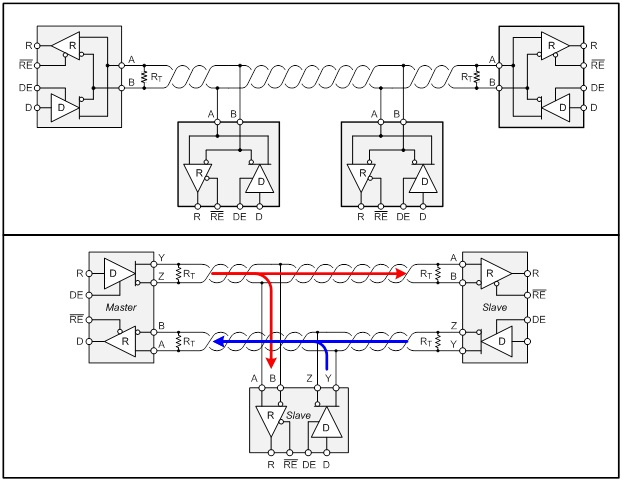
\includegraphics[scale=0.8]{images/rs485-fullduplex-halfduplex.jpg}
      \caption{Half-duplex and Full-duplex implementations}
      \label{fig:fullHalfDuplex}
      \end{center}
    \end{figure}


    Working principle of RS-485 is different in comparison to other standard; Instead of using a zero ground as the voltage reference, which will cause noise over the communication length, it uses floating voltage between two wires of the signal pairs, A and B or (+) and (-). After transmitting, the receiver compares the different of voltage between two wires and achieved the correct data with the lowest noise may cause. Figure~\ref{fig:rs485Wave} illustrates an example of the RS-485 waveforms transmitting one byte which has Mark, Space, and Idle phases. In most network, there will be one node acting as the master and the rest work as the slaves. At this point, the master sends command frame over the connection, and all slaves receive the data, then each slave with different functionality will work as programmed with different received data and also response to the master as programmed. The best practical result is obtained with the use of twisted pair of wires because some of the noise current will flow in the opposite direction with the current in the cable. In case using the straight cable, the noise current flows straightly along the cable in the same direction which will cause a loop current. Combined with the twisted pairs of wires, the cable also comes with shield, which is an accepted approach to restrain the noise, is used in applications that need higher noise resistance.
    \begin{figure}[!ht]
      \begin{center}
        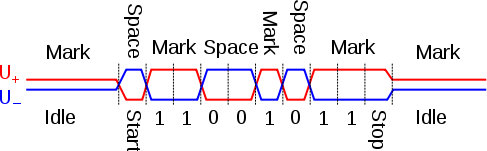
\includegraphics[scale=0.8]{images/RS-485_waveform.png}
        \caption{RS-485 waveform}
        \label{fig:rs485Wave}
      \end{center}
    \end{figure}

    As written in the introduction, RS-485 can connect with multiple transmitters and receivers in the same network. For instance, using input resistance around 12k\si{\ohm},the numbers of devices can connect to the system is up to 32. Besides, with the connecters, this number can increase significantly to the number of thousands and the transmitting distance can be also extended to kilometers. In addition, the network implemented with RS-485 needs termination, usually with a 120\si{\ohm} resistance at the end of two wires. This is applied to terminate or minimize the reflection in order to avoid the fraud of sending data. Furthermore, it usually included pull up and pull down resistors for fail-safe bias in each wire in case that any wire is not controlled by any device. When input voltage ranging from -200mV to +200mV, receiver understands as “undefined” state, which caused by several reasons such as system is shutdown, connection from receiver to network is lost, or cable has an open or short part. In this case, fail-safe biasing is applied in order to confirm that the receivers receive defined states only.

  \subsection{MQTT}
    MQTT is abbreviation of Message Queuing Telemetry Transport, which is a protocol laid in Application layer of OSI model. It is designed as a machine-to-machine and remarkably lightweight protocol that helps communication between constrained devices becomes effortless in comparison to other wireless protocols. In detail, its working principle based on publish and subscribe methodology in order to reduce the amount of transmitting data which leads to the reduction of used bandwidth, latency and power consumption.

    A \gls{mqtt} system is the combination of a server, but usually named broker, and the clients, in which can acts as either a publisher, subscriber or both. One broker can have numerous clients connect to and each client can subscribe to any topic it is programmed. These subscribers are following and watching for the changes of data of the subscribed topics, once other clients which are defined as the publisher publishes message to the topics, then the broker distributed the payload of message to other clients who had subscribed to those topics. In this scenario, the publisher and subscribers do not need to know the information of each other, the only needed are the topics for publishing and subscribing. Figure~\ref{fig:mqttEg} refers a simple example of a MQTT system consists of one broker and four clients, in which three clients are the publishers and one is the subscriber that subscribes to three topics the publishers publish to. To be specific, three publishers are the sensor nodes publish to three topics, temp1, temp2 and temp3; the last client named Sensor Data Gatherer acts as the subscriber that follows three topics mentioned previously. At once, the subscriber will receive the message whenever a publisher broadcasts the message to any of those topics. Implemented MQTT system will be described in details in later part of the thesis.
    \begin{figure}[!ht]
      \begin{center}
        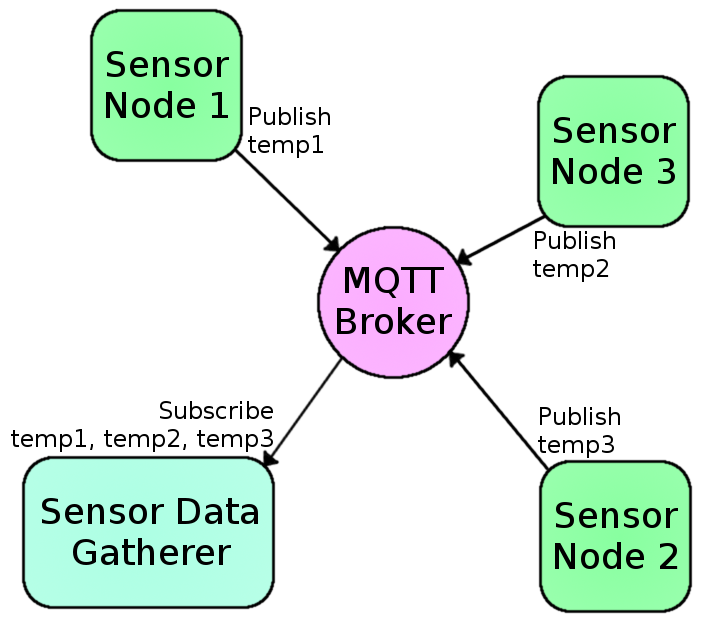
\includegraphics[scale=0.4]{images/mqttEg.png}
        \caption{Simple example of a MQTT system}
        \label{fig:mqttEg}
      \end{center}
    \end{figure}

  \subsection{WebSocket}
    WebSocket was introduced in 2011 in term of a communication protocol, implementing full-duplex channels over one TCP connection. The protocol is laid in Application layer of OSI model but distinguished from HTTP. Distinct to HTTP, in WebSocket applications, a server can send the data to client without waiting for requests from client. All data are being sent between server and client will be sent to a settled connection which helps accelerate the data rate and keep the connection opened when necessary. Similar to \gls{mqtt}, it is designed to reduce the transmitting data, which leads to the reduction of bandwidth and consumed power. Although it is designed for web applications, still, it can be implemented in any applications that need such a lightweight protocol.
    \begin{figure}[!ht]
      \begin{center}
        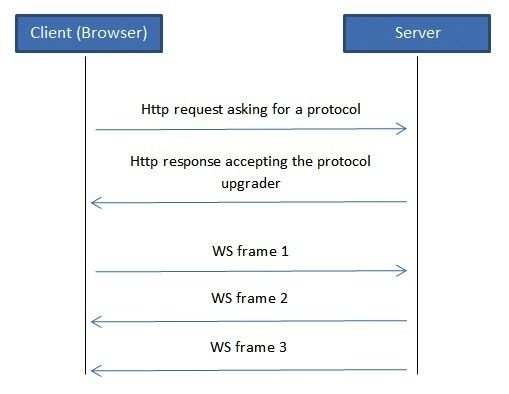
\includegraphics[scale=0.7]{images/ws-1.jpg}
        \caption{WebSocket working principle}
        \label{fig:wsPrinciple}
      \end{center}
    \end{figure}
    Figure~\ref{fig:wsPrinciple} illustrates how WebSocket works. There are two parts of the protocol, handshaking and transmitting data. At first, client sends a request to server to initialize the websocket connection, the server then send an acceptance to connect. After this point, the data are being sent as WS frame with numbering as in the Figure~\ref{fig:wsPrinciple}.

\section{Facial Recognition}
%TODO: finish facial recognition chapter
\section{Application Server}
%TODO:finish application server section




  



% \section{Test 2.1}
% \input{chapters/sections/sections2.1}
 
\chapter{Chapter Three Title}
\section{Expected System Diagram}
\begin{figure}[!ht]
    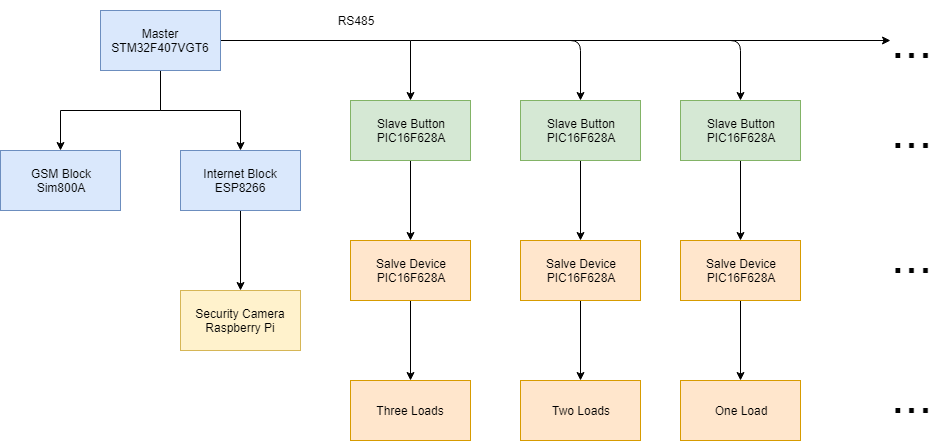
\includegraphics[scale=0.5]{images/hardwareBlock.png}
    \caption{Expected hardware blocks}
    \label{fig:hardwareBlock}
\end{figure}

    \begin{table}[h!]
    \begin{center}
    \begin{tabular}{ |c||c||c|  }
      \hline
      Attributes & Detail & Notes\\
      \hline
      Maximum number of devices&   99& Can be extended by\\
      & &extending command frame\\
      \hline
      Longest distance supported&   1200 meters&\\
      \hline
      Communication method &Mainly RS-485&\\
      \hline
      Wi-Fi connection & Wi-fi 2.4GHz&\\
      \hline
     \end{tabular}
     \caption{System ideal characteristics}
     \label{table:idealCharacteristics}
    \end{center}
    \end{table}
    In Figure~\ref{fig:hardwareBlock}, there are blocks named Master, Slave Buttons, Slave Devices, GSM block, Internet block and Security Camera. Each block is indicated with implemented hardware and how they connect to each other. As in the figure~\ref{fig:hardwareBlock}, Master is connecting with number of Slaves by UART over RS-485; Also, Master is implemented with GSM and Internet blocks in order to help end user controlling devices and receiving alerts over GSM or Wi-Fi. Each slave connects to the system has the same working principle but different names. In this thesis, there are two slave-2-devices and one slave-3-devices alongside with two slave-2-buttons and one slave-3-buttons to control the loads, respectively. Besides, the author designed one slave-2-buttons and one slave-1-button to control three out of seven existed devices. Three slave-devices are implemented with relays switch state for devices in the house, last device (Device 3) of slave-3-devices is assigned as the Main Door trigger to demonstrate the Security Camera System with Facial Recognition later on.

    Internet Block is the middle man for communicating between Application Server and the System. With this block implemented, end-user can control devices without pushing the physical buttons, which may causes difficulties for users because the owners can control their house whenever and wherever they want. Besides, with the help of the Application Server, end-users can collect and monitor data in the house in order to diagnostic and maintain precisely. GSM block should be installed in order to help in the event that Internet block is having unexpected problems.

    Security Camera block is the block that monitors the main door and inside the house. The camera installed outdoor is responsible for outdoor security in which it will track people entering the house with a facial recognition system. Additionally, indoor camera should handle the motion detection system while the owner is not at home in order to find strange motion which maybe a burglar breaking in the house. These two system will track and alert by emails, mobile application and text message over GSM network in the case that they detect something. Furthermore, the three-dots indicates that the system can be extended with number of slaves over RS-485, but only up to 99 dues to the limitation of command frame.
%Master hardware design
\section{Master}
    \subsection{Microcontroller Requirements}
    There are few requirements for the Microcontroller that the author decided to build the system for the thesis, listed as following.
    \begin{itemize}
        \item Support UART in order to communicate with other modules, namely RS-485, ESP8266 and SIM800A.
        \item Has widely support community.
        \item Easy to learn to program.
        \item Extendable with installed components.
        \item Price and ability for effortless replacement.
      \end{itemize}
      \begin{figure}[!ht]
        \begin{center}
        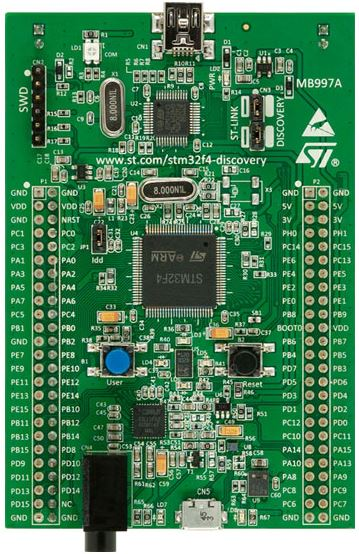
\includegraphics[scale=1]{images/stm32f4_discovery.jpg}
        \caption{STM32F4 Discovery Kit}
        \label{fig:stm32Kit}
        \end{center}
      \end{figure}
      Based on the requirements, the chosen MCU is STM32F407VGT6 with STM32F4 Discovery Kit from STMicroelectronics. Figure~\ref{fig:stm32Kit} refers the real kit in the market. It is considered as a suitable MCU because of the following reasons.
      \begin{itemize}
        \item The board has large support community.
        \item Programmed with C language with countless documents.
        \item MCU used is STM32F407VGT6, with core ARM Cortex 32bit M4, clock up to 168Mhz.
        \item Support up to 140 I/O.
        \item Flash memory 1MB.
        \item Easy to flash even with end-user.
        \item Cheap price and easy to find replacement parts.
      \end{itemize}
      \begin{figure}[!ht]
        \begin{center}
        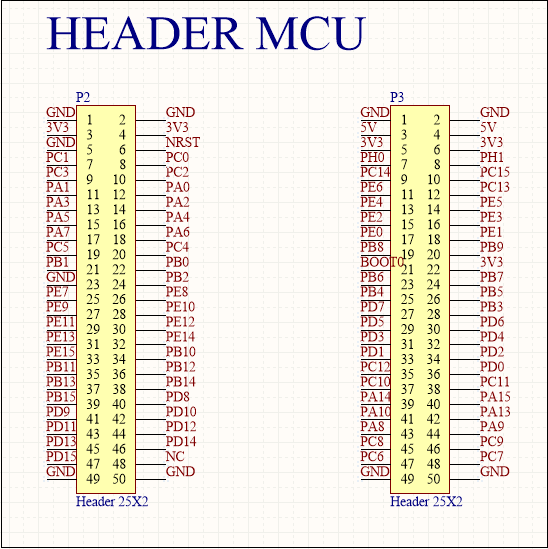
\includegraphics{images/headerMcu.PNG}
        \caption{Header for STM32F4 Discovery Kit}
        \label{fig:headerMcu}
        \end{center}
      \end{figure}
      In this thesis, to ensure the effortless replacement of the system parts, the author designed with modules attached on PCB by using headers. With this method, whenever an error occurs to any part of the system, end-user can replace the broken part easily without replacing the whole system. Figure~\ref{fig:headerMcu} shows the headers on Master board for STM32F4 Discovery Kit which is chosen for the thesis. In addition, it shows the connection pin of the MCU with other modules over UART. To be more specific, MCU connects with RS-485 module over UART1 via pin PB6-PB7, with module ESP8266 over UART2 via pin PD5-PD6, with module SIM800A over UART3 via pin PD8-PD9.
      %hardware RS-485
      \subsection{Module RS-485}
      \begin{figure}[!ht]
        \begin{center}
        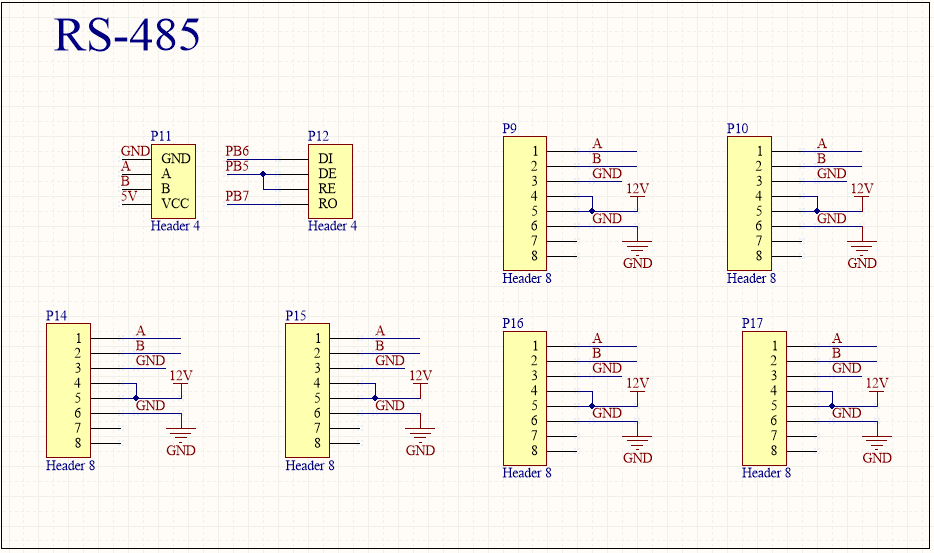
\includegraphics[scale=0.63]{images/header485.PNG}
        \caption{Header for module RS-485}
        \label{fig:header485}
        \end{center}
      \end{figure}
      \begin{figure}[!ht]
        \begin{center}
        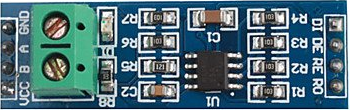
\includegraphics[scale=1]{images/module-rs485.png}
        \caption{Module RS-485}
        \label{fig:module485}
        \end{center}
      \end{figure}

      Figure~\ref{fig:module485} refers the cheap version of module TTL to RS-485 on the market. It integrated IC MAX485 as the main component and other sub-components included termination resistor. This module is stable enough for the system and easy to replace due to its cheap price but does has a weakness which is if it is broken, end-user cannot know unless further tests on the module is processed. The table~\ref{table:module485PinOut} indicates the pin out guideline to connect with the MCU. According to datasheet of IC MAX485, RE and DE must be connected for the MCU to control the module based on logic level, in which the module is transmitting if the pins are pull up to 1, otherwise it is receiving.
      \begin{table}[h!]
        \begin{center}
        \begin{tabular}{ |c||c|  }
          \hline
          Pin & Detail\\
          \hline
          VCC& 5V\\
          \hline
          A&   Non-inverting Receiver Input and Non-inverting Driver Output\\
          \hline
          B &.Inverting Receiver Input and Inverting Driver Output\\
          \hline
          GND & GND, should be 0V\\
          \hline
          RO & Receiver Output (to Rx pin of microcontroller)\\
          \hline
          RE & Receiver Output Enable (Low to enable)\\
          \hline
          DE & Driver Output Enable (high to enable)\\
          \hline
          DI & Driver Input (to Tx pin of microcontroller)\\
          \hline
         \end{tabular}
         \caption{Module UART TTL to RS-485 pin out}
         \label{table:module485PinOut}
        \end{center}
        \end{table}
      
      Figure~\ref{fig:header485} shows the headers which are used on Master board for RS-485 module in figure~\ref{fig:module485} and the headers of RJ-11 female jack for RS-485 output of the Master. The reason for choosing RJ-11 jack and its compatible cable is the cable suits for the project which needs four wires, in which two are the signal wires (A and B of RS-485 standard) and the other two are the pair providing power for other slaves (12V and GND). With this method, a four-wire twisted cable with shield is used in order to keep the noise as low as possible and still, provides the power along the whole system with only one cable connected.

      \subsection{Module ESP-8266}
      This module is implemented to establish the connection between the Application Server and the System. End-users can control and monitor their system with a website or an android application over Wi-Fi connection with module ESP-8266. There are various versions of module using ESP-8266 on the market, but the full name of the chosen module is ESP-8266 NodeMCU lua CP2102. It is a small size kit that integrated with ESP8266 SoC, other components and it is also compatible with Arduino IDE which makes it become the easiest to use ESP-8266 module in comparison to other versions.
      \begin{table}[h!]
        \begin{center}
        \begin{tabular}{ |c||c|  }
          \hline
          Attribute & Detail\\
          \hline
          SoC& ESP8266 Wifi SoC\\
          \hline
          Firmware&   NodeMCU Lua\\
          \hline
          Flash chip &CP2102\\
          \hline
          GPIO & compatible with firmware of Node MCU\\
          \hline
          Power supply & 5V DC with Micro USB or Vin\\
          \hline
          GPIO logic level & 3.3V\\
          \hline
          Integrated LED & Reset, Flash and Status indicator\\
          \hline
          Dimension & 25mm x 50mm\\
          \hline
          Others& Compatible with Arduino IDE\\
          \hline
         \end{tabular}
         \caption{Module ESP-8266 NodeMCU lua CP2102 remarkable characteristics}
         \label{table:moduleEspDetail}
        \end{center}
        \end{table}

        \begin{figure}[!ht]
            \begin{center}
            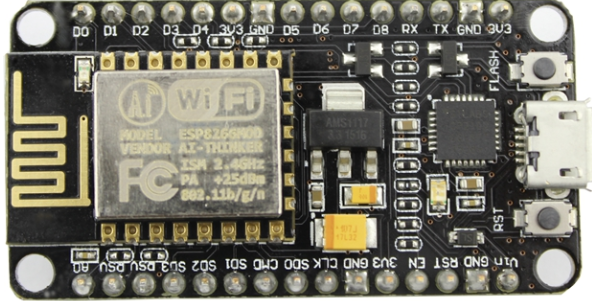
\includegraphics[scale=0.9]{images/module-esp.png}
            \caption{Module ESP-8266 NodeMCU lua CP2102}
            \label{fig:moduleEsp}
            \end{center}
          \end{figure}

          \subsection{Module SIM800A}
          %TODO: finish module SIM800A

          \subsection{Power for Master}



 
\chapter{Chapter Four Title}
\section{Features explanation}
    In this thesis, the system must have the ability to control devices in the house in a convenient way, which means user can control devices from anywhere, anytime they want with an Internet-connected device and timer. Furthermore, the house should be capable of providing scenarios depends on the needs of user. For instance, users can switch on or off a number of specific devices by choosing a scenario instead of choosing individual device, namely “I’m home”, “Good night”, or “I’m leaving”. Based on the basic ideas, the thesis is integrated with all the basic features above. The thesis is designed for an one-floor house with three rooms, namely Living Room, Dining Room and Bedroom.
    \subsection{Convenient control}
    \subsubsection{Living Room}
    Front part of the house, which includes Main Door, Living Room and a Stair, the belonging AC devices will be controlled with four Relays but integrated into two Slave-Relay(s), one is Slave-3-Relays and the other is Slave-2-Relays (which is also integrated with the Relay controlling the Conditioner of Bedroom).
    \subsubsection{Dining Room}
    Second part of the house is assumed to have only one AC device and will be controlled with a Relay integrated on a Slave-2-Relays, in which has the Relay to control the Bedroom Light.
    \subsubsection{Bedroom}
    Last room of the house is Bedroom, in which is assumed to have two devices but one is integrated on the same circuit with Dining Room Light, the other is the Conditioner is also integrated on the same circuit with the Living Room Light.

    Apart from controlling the devices by physical Slave Button(s), which is also crossed implemented with no specific rule, the owner also can control the devices with a single Internet-connected device such as a smartphone, a tablet or a computer by accessing the Web Server from anywhere and anytime. Besides, it also has few scenarios that should be quite helpful for the owner. Imagine that when the owner arrive home after work, the devices needed are ready to serve such as the Front Light or the Conditioner. The project is also implemented with security camera block which helps user to access, monitor their house and receive alert in case of abnormal event happens in a convenient way with reasonable price. In addition, all data in the process of monitoring the house should be sent to a database, which helps the user and also engineer can keep track of the activities of devices in the house, then use the collected data to improve the experiences of the users in the future.

    \subsection{Block Diagram}

    \begin{figure}[!htp]
        \begin{center}
        \includegraphics[scale=0.55]{images/systemFullBlock.PNG}
        \caption{System Block Diagram}
        \label{fig:blockDiagram}
        \end{center}
    \end{figure}
    Figure~\ref{fig:blockDiagram} refers the overview of the system. From the block diagram, there are three main blocks, namely Master, Slaves and Internet Application block. In this thesis, each main block has different functions and may consists of one to many smaller blocks. Referring to Figure~\ref{fig:blockDiagram}, Master is in the middle, connects Slaves and Internet Application Block; Slaves are the “workers” depend on the Master and the Internet Block helps the User communicate with the system through Master remotely.
    \subsubsection{Master}
    As designed in section \ref{masterDesign}, Master is the circuit integrated with a STM32F4 Discovery Kit, connected via headers instead of being soldered directly on board in order to ensure an effortless replacement if broken. Beside the block of RS-485 module for main communication methodology and ESP-8266 for establishing connection to the Internet, it also has the headers for other modules of connectivity and functions in order to make the Master scalable in the future, namely SIM800A, Bluetooth module HC-05, and Real time module DS3231. However, instead of using an integrated Power block onto Master circuit, it uses a separated Power for Master as mentioned in section \ref{powerForMasterDesign}.

    Based on the basic idea, Master is responsible for receiving the requests from all sources, Slaves or Internet Application block, and distributing the command to the Slave with appropriate function. In addition, Master is also the middleman between Internet Application block with the Slaves, which means it also update the information between Internet application block and Slaves.
    \subsubsection{Slave Relay(s)}
    Slave Relay(s) (Slave \#1, \#2, \#3) consists of number of Relays (varies depends on users’ needs) and one PIC16F628A from Microchip as the MCU, responsible for switching AC devices On or Off based on the distributed command from Master.
    \subsubsection{Slave Button(s)}
    Slave Button(s) (Slave \#4-8) consists of number of Buttons (varies depends on users’ needs) and one PIC16F628A from Microchip as the MCU, responsible for controlling Slave Relay(s) by sending the commands to Master for the distribution to corresponding Slave Relay(s).
    \subsubsection{Internet Application Block}
    Internet Application block consists of smaller blocks with different functions, namely Database, Web Server, Internet connection block, Security Camera and Smart devices. Internet block establish the Internet connection for Master block; Web Server is the combination of back-end and front-end development of Webserver, besides helping users to control the system remotely with ease, the extended features will be explained later in this chapter; Security Camera responsible for recognizing person with Facial Recognition to open the door in order to cut off the steps of accessing the house. In addition, security camera is also integrated with motion detector prototype directly in Web Server. The Web Server communicates with the system through Internet block using MQTT protocol.

    \section{Communication Methodology and Algorithm of Master and Slaves}
    In this thesis, data is transmitted from UART of MCU to input of module RS-485 then to the data bus wire to distribute to corresponded components, noted that RS-485 is the physical standard which helps transmitted data travels much further compared to original UART. It needs two wires for data transmitting with module RS-485, but a cable of four wires is chosen for providing power supply of 12VDC and transmitting data at the same time with a single cable. Four wires in a cable with corresponded functions are listed as following.
    \begin{itemize}
    \item 12V: provide 12VDC throughout the system.
    \item A: Signal wire A.
    \item B: Signal wire B.
    \item GND: Common ground throughout the system.
    \end{itemize}

    However, RS-485 is a physical standard instead of an algorithm to distribute data through the whole network of a large number of devices with acceptable performance. Furthermore, in order for the chosen module RS-485 be able to work, its enable pin must be controlled by the MCU, which is set to logic 0 as default is receiving mode and vice versa. After sometimes reading books, the author suggested two algorithms for this thesis.
    \subsubsection{Ask/Request sequentially}
    \begin{itemize}
    \item \textbf{Master}: Master responsible for asking sequentially every connected Slaves in the system. After asking the Slaves for if they need to work, Master will delay for a small amount of time to wait for the response from Slaves. If the time is passed and asked Slave does not request to work, Master will pass that Slave and move on the next Slave. If a Slave Button is being asked but also receive the external signal, it can interrupt the process by sending a response to Master requesting to work, then that request will be prior to be sent to corresponded Slave Device. Now it ends the loop and start a new one. Period of time to ask the Slaves must be in milliseconds in order to complete the loop for every Slaves in the system.
    \item \textbf{Slave Button}: Slave Button has to wait for Master to ask and response. It is always stay in receiving mode (which has enable pin logic at 0 – LOW). When Slave Button is asked or an external signal comes in, it pulls enable pin to logic 1-HIGH to enter transmitting mode and response when Master asks.
    \item \textbf{Slave Device}: Enable pin of RS-485 of Slave Device is always in LOW status, which means receiving data mode. When Master ask or there is data transmitted from Slave Button, Slave Device will check if it is corresponded with its functions, if yes Slave Device will work as defined function.
    \end{itemize}
    
    With this algorithm, the asking loops will run continuously, and it should prevent two signal collide with one and another because the Slave only answers Master when Master asks. However, transmitted data will be difficult to be managed because of two reasons, waiting time and management. After a request is sent from Master, it takes some time for Master to wait for the response from Slave and pull enable pin of RS-485 to LOW. Besides, it takes times again to pull enable pin up to logic HIGH to distribute the response if available. This process is getting longer with the increment of the number of Slaves, which cause the transmission between Slaves become slower with a large number of Slaves. Furthermore, transmitting data continuously will consume loads of bandwidth leads to resource waste and cause errors dues to noise or inaccurate process from Slaves because of data is transmitted continuously leads to false data or worse is lose data. Thus, the author chose a different method to transmit data through the network based on CSMA/CD protocol.

\subsubsection{Work sequentially}
Based on the idea of CSMA/CD protocol, which is “Carrier-sense multiple access with collision detection”. It is explained briefly as if a node need to transmit data, it has to listen if the connection is busy or not. In the case the connection is idle, frame is transmitted, if not, that node has to wait a random time then start to listen again. In order to detect collision, transmitting node has to listen to the connection while transmitting data. If a collision is detected, that node has to stop transmitting and send a jam signal to others station while waiting a random time to start sending frame again.
In this thesis, the algorithm is built based on the working principle of CSMA/CD and Master-Slave model.
    \begin{itemize}
    \item \textbf{Master}: Master is the most important node in the network. After the system is booted up, Master will be ready and waiting for the transmission. The author could not complete the idea to set an identity for a new Slave entering the network, therefore, all identity will be pre-programmed and managed by the Master. Master now responsible as a middleman, receiving and distributing frames between Slaves in the network. Whenever a Slave Button send a frame to control assigned Slave Relay, Master will receive the frame then distributed to corresponding Slave Relay without a direct connection between any Slaves. With all the process, Master will pull up RS-485 to 1-HIGH when transmitting frame or pull down to 0-LOW (as default) when receiving frame.
    \item \textbf{Slave Button}: Slave Button will be in receiving mode (enable pin of RS-485 is 0-LOW) after booting up. When a button is pressed, it will pull up enable pin of RS-485 to 1-HIGH and send corresponding frame to Master for the distribution to the correct Slave Relay with corresponding identity. Then it returns to receiving mode to wait for the interruption again.
    \item \textbf{Slave Device}: Enable pin of RS-485 of Slave Device is always in LOW status, which means receiving data mode. When there is data transmitted from Slave Button, Slave Device will check if it is corresponded with its functions, if yes Slave Device will work as defined function.
    \end{itemize}

With this algorithm, Master will update Slave status after booting up, then Master and Slaves enter receiving mode to listen to transmission. It is an improvement in processing time and management compared to the previous algorithm. To be specific, frames are not transmitted relentlessly which saves large amount of resources and the delay is almost unnoticeable, this leads to the project can be extended to a number of slaves without much delays. Furthermore, the transmission is free in default, thus minimizes the chance that there will be two frame on the connection at the exact same time, this helps the frame is transmitted correctly with small probability that a collision is happened.

\subsection{Transmitting Frame Design}
    \subsubsection{Master to Slave Relays}
    In this thesis, a standard transmitting frame consists of 11 bytes as following.

    \begin{center}
    S$X_1$$X_2$$X_3$$X_4$$X_5$$X_6$$X_7$$X_8$$X_9$E
    \end{center}

    \textit{Explanation}:
    \begin{itemize}
        \item S: For recognition that a Frame is being transmitted.
        \item $X_1$: For recognition that the Master is transmitting to a Slave or vice versa. For instance, $X_1$=1 is Master transmits to Slave and $X_1$=0 is Slave transmits to Master.
        \item $X_2$: Byte for defined function. In this thesis, $X_2$=0 is the command controlling assigned Relay with a defined Button. $X_2$ has range from 0 to 9, which means the functions for the project can be extended up to 10 functions if necessary. 
        \item $X_3$$X_4$$X_5$: Bytes define identity of each component on Slave Relays or Slave Buttons. For instance, D01 is Relay number 1 (integrated on Slave-3-Relays in this thesis) or B02 is Button number 2 (integrated on Slave-3-Buttons in this thesis).
        \item $X_9$: Byte defines state of the device on Slave Relay which is being controlled. For instance, $X_9$=1 is “Turn device On” and $X_9$=0 is “Turn device Off”.
        \item $X_6$$X_7$$X_8$: Bytes that are reserved for further development.
        \end{itemize}

    \subsubsection{Slave Button to Master frames}
    Frame from Slave Buttons to Master is slightly different from frames from Master to Slave Relays.

        \begin{center}
        S$X_1$$X_2$$X_3$$X_4$$X_5$$X_6$$X_7$$X_8$$X_9$E
        \end{center}

    \textit{Explanation}:
    \begin{itemize}
    \item S: For recognition that a Frame is being transmitted.
    \item $X_1$: For recognition that the Master is transmitting to a Slave or vice versa. For instance, $X_1$=1 is Master transmits to Slave and $X_1$=0 is Slave transmits to Master.
    \item $X_2$: Byte for defined function. In this thesis, $X_2$=0 is the command controlling assigned Relay with a defined Button. $X_2$ has range from 0 to 9, which means the functions for the project can be extended up to 10 functions if necessary. 
    \item $X_3$$X_4$$X_5$: Bytes define identity of each Button on Slave Button. For instance, B01 is Button number 1 (integrated on Slave-3-Buttons in this thesis) or B04 is Button number 4 (integrated on Slave-2-Buttons in this thesis).
    \item $X_6$$X_7$$X_8$: Bytes define identity of each Relay on Slave Relays, which is the part to identify which Relay the Button needs to control. For instance, D01 is Relay number 1 (integrated on Slave-3-Relays in this thesis) or D02 is Relay number 2 (integrated on Slave-3-Relays in this thesis).
    \item $X_9$: Byte defines state of the device on Slave Relay which is being controlled. For instance, $X_9$=1 is “Turn device On” and $X_9$=0 is “Turn device Off”.
    \end{itemize}

    \begin{figure}[!h]
        \begin{center}
        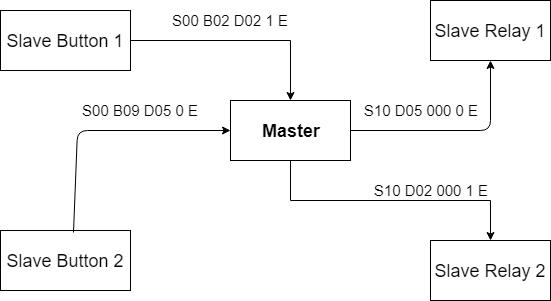
\includegraphics[scale=0.75]{images/frameEx.png}
        \caption{Example of transmitting frames}
        \label{fig:frameEx}
        \end{center}
    \end{figure}

    In particular, Figure~\ref{fig:frameEx} shows an example of frames transmitting in the system with the explanation above. The case of Slave Button 1 sends the frame of \textbf{S00 B02 D02 1 E} and Master sends a frame of \textbf{S10 D02 000 1 E} to Slave Relay 2 is explained in detail as following.
    \begin{itemize}
        \item S: For recognition that a Frame is being transmitted.
        \item $X_1$ = 0 indicates Slave Button 1 is sending to Master.
        \item $X_2$ = 0 indicates Slave Button 1 wants to control a Relay with the identity as of bytes $X_6$$X_7$$X_8$.
        \item $X_3$$X_4$$X_5$ = B02 indicates Button number 2 is controlling.
        \item $X_6$$X_7$$X_8$ = D02 indicates Button number 2 is controlling Relay number 2.
        \item $X_9$ = 1 is “Turn device On”.
    \end{itemize}

    \subsection{Working flowchart of Master and Slaves}
    In this section, the author shows the flowcharts of programs that are embedded in Master and Slaves. Each flowchart has a description below corresponding to its design. For instance, figure~\ref{fig:masterFlow}, figure~\ref{fig:buttonFlow} and figure~\ref{fig:relayFlow} indicates working principle of Master, Slave Button and Slave Relays, respectively.
    \begin{figure}[!htbp]
        \begin{center}
        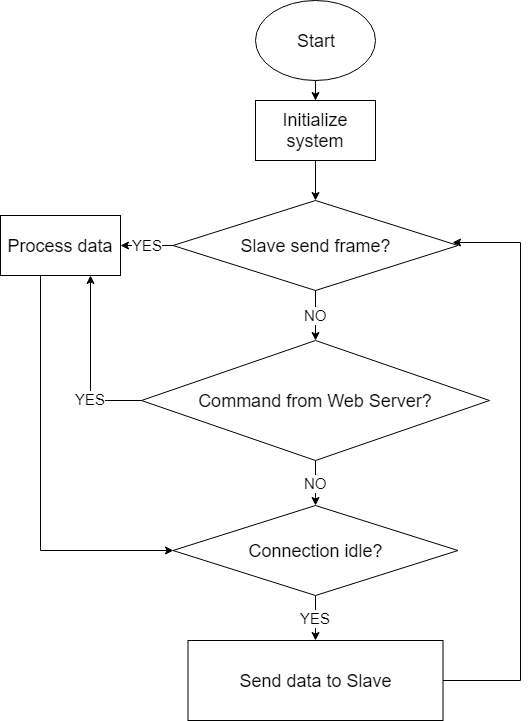
\includegraphics[scale=0.75]{images/masterFlow.png}
        \caption{Flowchart of Master}
        \label{fig:masterFlow}
        \end{center}
    \end{figure}
    \begin{figure}[!htb]
        \begin{center}
        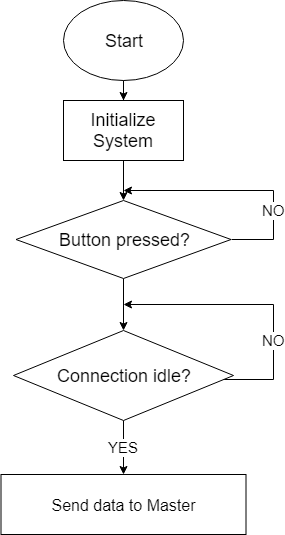
\includegraphics[scale=0.55]{images/buttonFlow.png}
        \caption{Flowchart of Slave Button}
        \label{fig:buttonFlow}
        \end{center}
    \end{figure}
    \begin{figure}[!htb]
        \begin{center}
        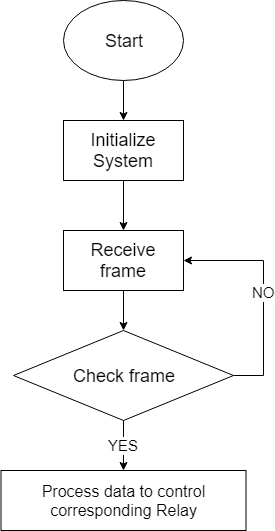
\includegraphics[scale=0.55]{images/relayFlow.png}
        \caption{Flowchart of Slave Relay}
        \label{fig:relayFlow}
        \end{center}
    \end{figure}

\newpage
\section{Internet Application Block Design}
Nowadays, Internet connection with its applications is the must have function for any smart system. This thesis is not fully implemented with Internet applications but the author chose the basic function that can support any user to live and control their house in an effortless way.
    \subsection{Internet Block} %esp8266
    In this thesis, Internet Block helps the user interact with the system through Wi-Fi connection with module NodeMCU ESP-8266. Beside establishing a connection between the Web Server and the system, it also handles the processing data phase in order to send a frame to Master.
        \subsubsection{MQTT Protocol}
        As for the connection between NodeMCU ESP-8266 and the Web Server, the author use MQTT protocol instead of HTTP. MQTT is an extremely lightweight protocol, designed for constrained devices. The topics for are designed with multiple levels to suits with the control methodology. For instance, NodeMCU is assigned as a client, which subscribes to the topic as shown in Figure~\ref{fig:espSub}.
        \begin{figure}[!htb]
            \begin{center}
            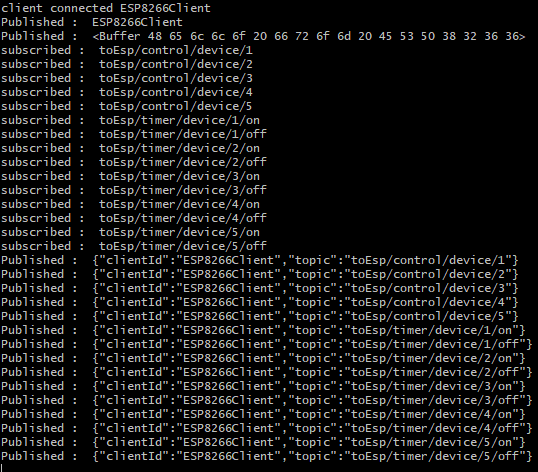
\includegraphics[scale=0.9]{images/espSub.png}
            \caption{Topics subscribed by NodeMCU}
            \label{fig:espSub}
            \end{center}
        \end{figure}

        \begin{figure}[!htbp]
            \begin{center}
            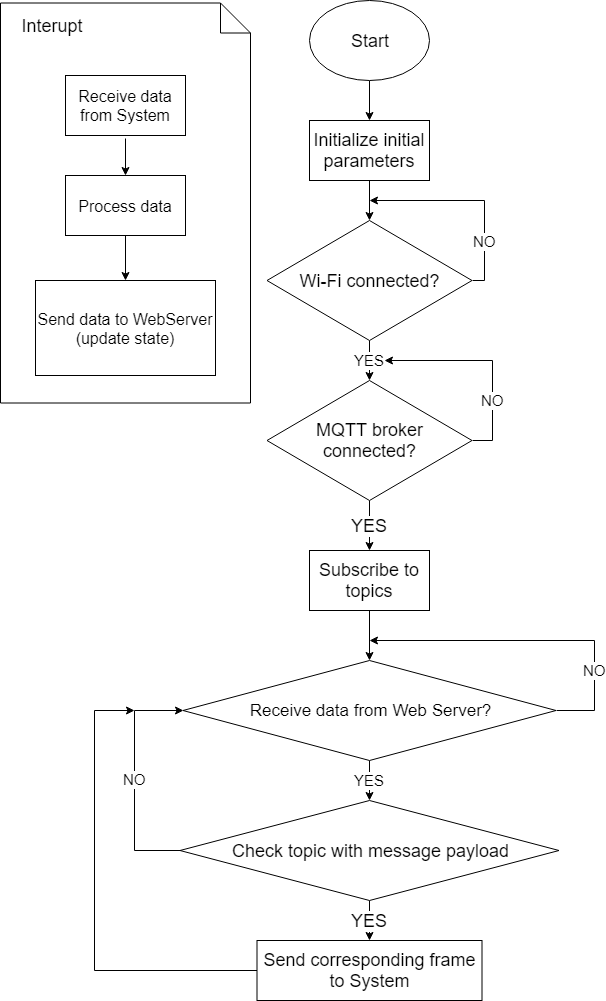
\includegraphics[scale=0.65]{images/mqttFlow.png}
            \caption{Flowchart of working principle of NodeMCU}
            \label{fig:mqttFlow}
            \end{center}
        \end{figure}
        In order to process the received data from Web Server, the author embedded a simple program for NodeMCU and Figure~\ref{fig:mqttFlow} illustrates its working principle.

    \subsection{Web Server}
    Web Server is the combination of Back-end and Front-end Design. To be specific, Back-end is the core for a Web Server which handles the logic and working flow of all components, Front-end is responsible for displaying the results of back-end processes and components to interacts. The author use Node.js for Back-end design and HTML, CSS for Front-end design.
        \subsubsection{Back-End Design}
        Node.js works on non-blocking I/O principle which makes it suitable for real-time applications included a real-time Web Server. Node.js empowers real-time web application by adopting push technology as against web sockets to build server-side web applications with two-way channel i.e. client and server. It operates on open web stack technologies like JavaScript, CSS, and HTML that work over the standard port 80. This tool is also lightweight both for in-memory usage and data dense real-time web applications that work on multiple devices. Figure~\ref{fig:nonBlocking} refers the working principle of Node.js in order to show its advantages for the Web Server in this Thesis.
        \begin{figure}[!htb]
            \begin{center}
            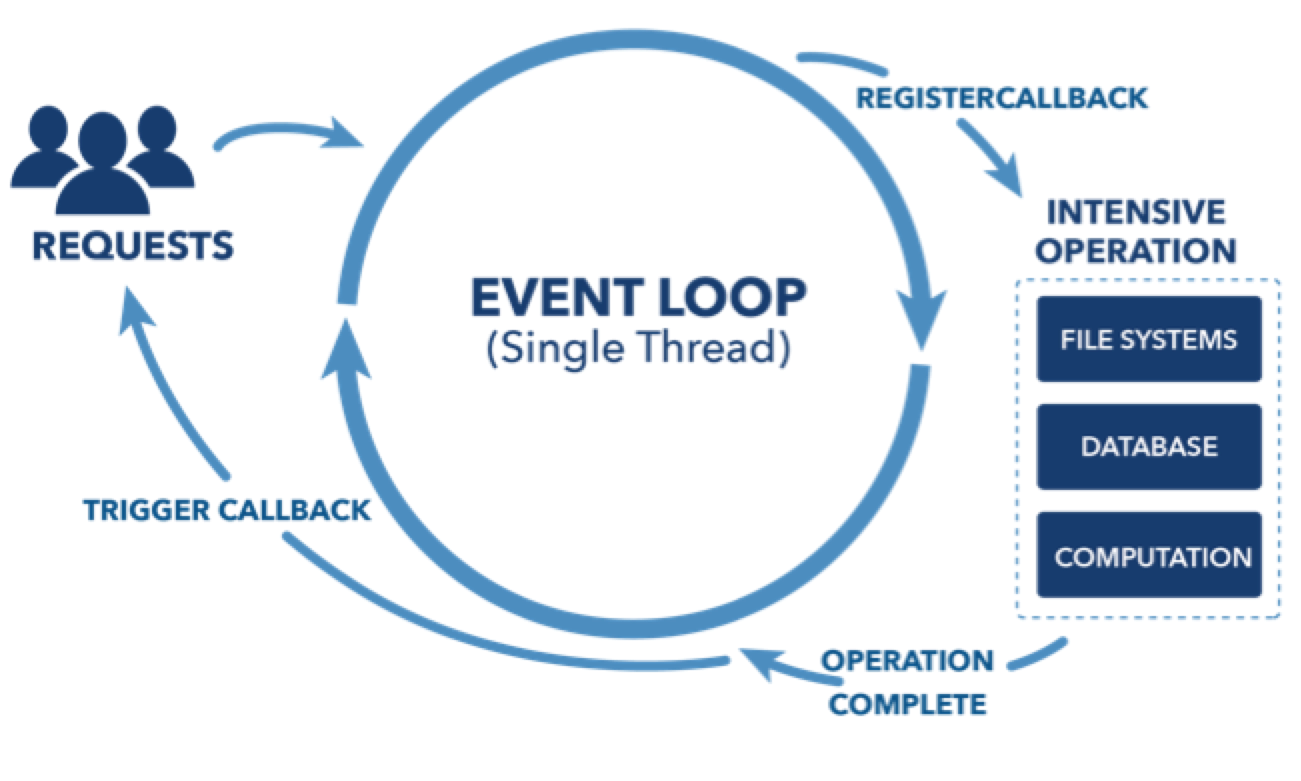
\includegraphics[scale=0.65]{images/nonBlocking.png}
            \caption{Node.js Working Principle}
            \label{fig:nonBlocking}
            \end{center}
        \end{figure}

        Server-side is implemented on port 2111 with MQTT protocol to communicate with other nodes in the network to control the system. In this thesis, the MQTT broker is running on port 3000 and written in Node.js using a module named Mosca, which makes a local and private Broker to implement MQTT protocol on. Figure~\ref{fig:webSub} shows the subscription of the Web Server to those topics which are in use of the Thesis.
        \begin{figure}[!htb]
            \begin{center}
            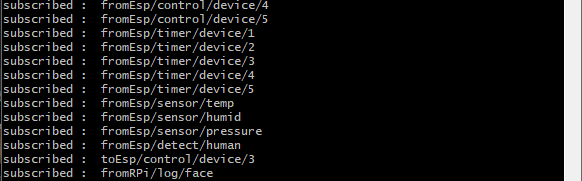
\includegraphics[scale=1]{images/webSub.png}
            \caption{Topics subscribed by Web Server}
            \label{fig:webSub}
            \end{center}
        \end{figure}

        In the Web Server, the author used both POST and GET methods in an appropriate way to ensure the sensitive information will not be exposed. For instance, the author used POST method for Log in information at Log in Page in order to make the information is not queried in the URL and GET method for getting page response to the Client.

        Because Web Server is an asynchronous application, it returns response to client whenever it receives a request from Client-side. After a successful log in session from the authorized person from the family, which means a default request is sent to Server-side to load the next page, Web Server is divided into four main pages corresponded to four function blocks, namely Dashboard, Control, Scenario and Indoor Security Camera. The activities of the devices will be logged into a Database, which helps to back up the data to monitor and should be used for future development. The figure~\ref{fig:responseBlock} illustrates the flowchart of every function blocks are implemented in this thesis that returns the corresponding response to Client-side.
        \begin{itemize}
            \item Dashboard: in this thesis, Dashboard page shows the overview of the system, namely the Sensor value (in the event a Slave Sensor is implemented) and Security Status of the Indoor Security Camera. Each component on this page will automatically retrieve the value from the Database, which is logged from the system in prior, and display for users with Front-end design.
            \item Control: Control page consists of the Button which help users to control devices on Slave Relay without pressing the physical buttons on Slave Buttons. This page is implemented with MQTT protocol to send command to the system and to receive state update from the system. Besides, a connection to the Database is also opened in order to log devices’ activities to monitor, maintain and develop in the future. The payload of the control message which is sent to corresponded topics is shown in the figure~\ref{fig:mqttPayload}. For instance, On is shown as “Buffer 6f 6e” and Off is “Buffer 6f 66 66”.
            \item Scenes: This page is implemented with four scenarios, namely Good Morning, I’m Home, Good Night and Security. The idea for this page is use the defined Scenarios to switch number of device On or Off in order to reduce the control time in similar circumstances. This page is also implemented with MQTT and a connection to Database to work as the same as Control Page.
            \item Indoor Security Camera: This page is a prototype implemented with Motion Detector using integrated WebCam of the computer. When the owner leaves the house, this function should be turned on and will be ready to detect the strange motion in an ideal condition that the house does not have any person or pet at home. If a motion is detected, it will send alert to the owner over Email and alert messages in all Pages if the Web Server is currently accessed by an authorized user, or in further development should be text messages over cellular network. It is also implemented with a connection to the Database to log the data in case of use in the future. The motion detection algorithm is done on Client-side, Server-side is responsible for receiving post-process data to raise alert in the event of strange motion occurs.
            \end{itemize}

        \begin{figure}[!htb]
            \begin{center}
            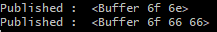
\includegraphics[scale=1.5]{images/mqttPayload.png}
            \caption{Control messages shown as Buffer Payload in corresponded topic}
            \label{fig:mqttPayload}
            \end{center}
        \end{figure}
        \begin{figure}[!htb]
            \begin{center}
            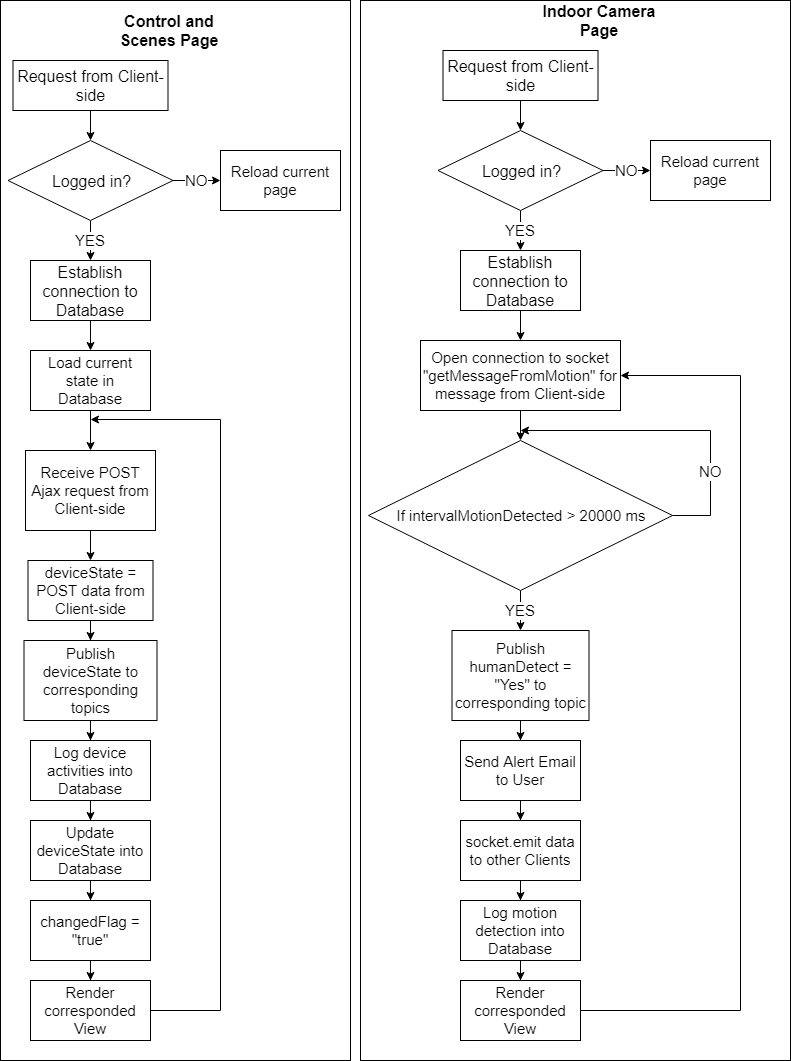
\includegraphics[scale=0.53]{images/responseBlock.png}
            \caption{Flowchart of each function blocks in Web Server}
            \label{fig:responseBlock}
            \end{center}
        \end{figure}

        \newpage
        \subsubsection{Front-End Design}
        Front-end design is the combination of languages, namely Javascript, HTML5 and CSS. With Node.js, the author is able to write both back-end and front-end in Javascript, which helps reduce plenty of time. Front-end design particularly means design the \gls{hmi} and the communication between Client-side and Server-side with Ajax technique, tools and libraries, namely jQuery, Bootstrap or Socket.io, which should help end-user interact with the application in an effortless way. The result of HMI will be shown in Chapter \ref{result}. Besides, Motion detection algorithm is shown as in figure~\ref{fig:motionFlow} and it is done in Client-side.
        \begin{figure}[!h]
            \begin{center}
            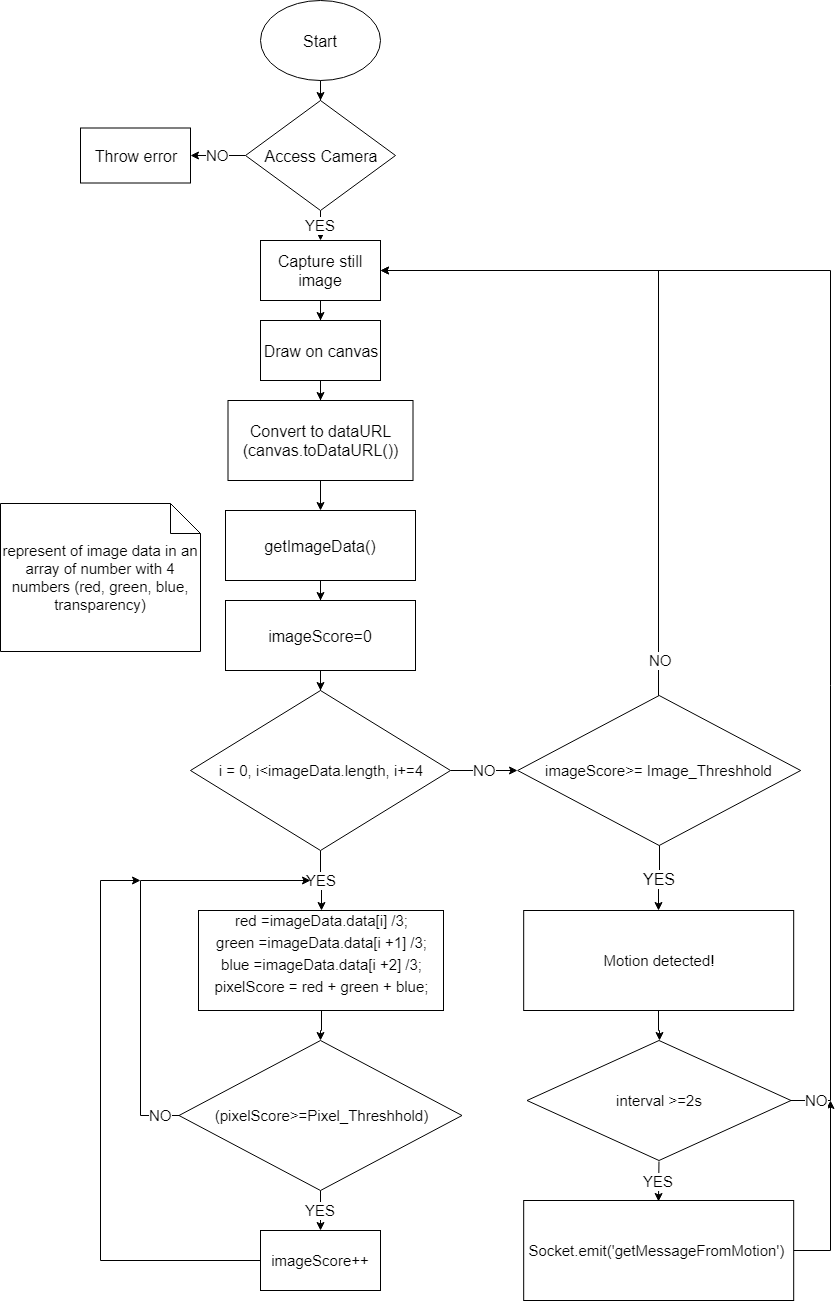
\includegraphics[scale=0.45]{images/motionFlow.png}
            \caption{Flowchart of Indoor Security Camera}
            \label{fig:motionFlow}
            \end{center}
        \end{figure}

    \subsection{Database}
    Database is a collection of data, create and managed in relational or non-relational way. In this thesis, the author chose MongoDB, a non-relational database. The database works similar to an electronic warehouse where data is organized and kept in categories and value by using key/value pair. To be specific, MongoDB stores data in BSON file, which is similar to JSON format, therefore easy to manipulate the stored data.

    In this thesis, the author organizes data with four collections, namely floor1, logDeviceActivities, logFaceDetection and logMotion. Each collection responsible for logging corresponding data. To be specific, floor1 stores all devices in houses with their id, name and state. In addition, logDeviceActivities, logFaceDetection and logMotion have timestamp in details to identify the time of any interaction with the house and its devices. Furthermore, logDeviceActivities and logFaceDetection also show deviceId with its State and person who accessed with the permission at the same time, respectively. Please see the figure~\ref{fig:floor1}, figure~\ref{fig:logDevice}, figure~\ref{fig:logFace} and figure~\ref{fig:logMotion} for the key/value pair of each collections.
    \begin{figure}[!ht]
        \begin{center}
        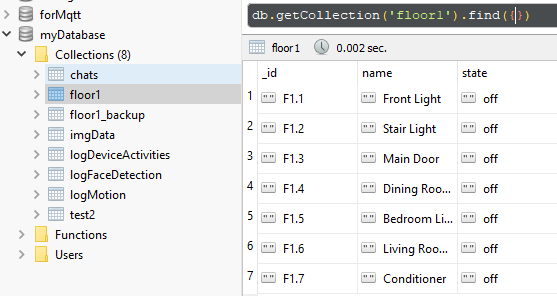
\includegraphics[scale=0.8]{images/floor1.png}
        \caption{Data of collection Floor1}
        \label{fig:floor1}
        \end{center}
    \end{figure}
    \begin{figure}[!ht]
        \begin{center}
        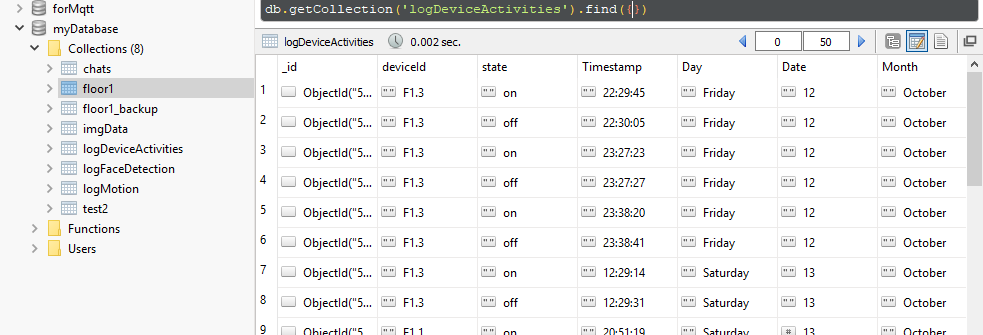
\includegraphics[scale=0.55]{images/logDevice.png}
        \caption{Data of collection logDeviceActivities}
        \label{fig:logDevice}
        \end{center}
    \end{figure}
    \begin{figure}[!ht]
        \begin{center}
        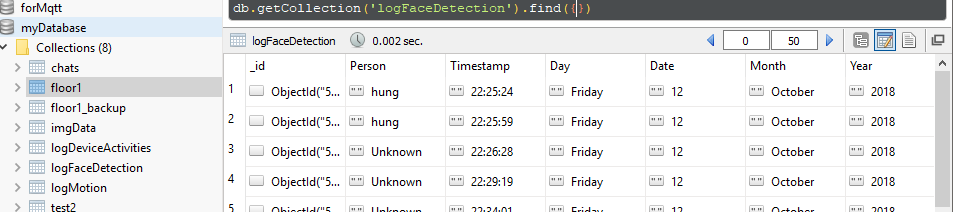
\includegraphics[scale=0.55]{images/logFace.png}
        \caption{Data of collection logFaceDetection}
        \label{fig:logFace}
        \end{center}
    \end{figure}
    \begin{figure}[!ht]
        \begin{center}
        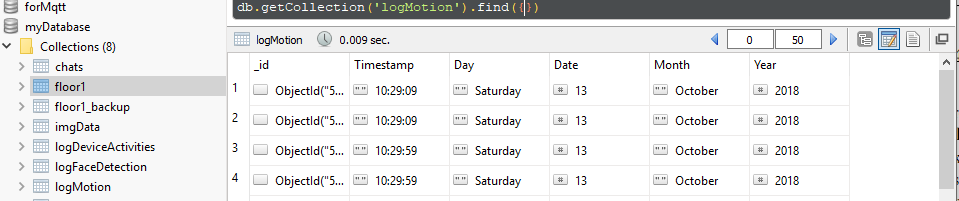
\includegraphics[scale=0.55]{images/logMotion.png}
        \caption{Data of collection logMotion}
        \label{fig:logMotion}
        \end{center}
    \end{figure}
 
    \subsection{Security Camera Block}
    Security Camera Block is implemented in the minicomputer named Raspberry Pi 3 Model B. The programme is written in python and implemented with OpenCV for Facial Recognition, in which OpenCV is a library aimed at real-time computer vision projects. Raspberry Pi 3 is installed with Raspbian OS and attached PiCamera Module via CSI port. With the help of OpenCV, the author is able to implemented a real-time facial recognition system with acceptable results. Because it is implemented in Raspberry Pi, the security camera block is capable of running full time when setup at front door with a power supply and a small monitor. Because the author is limited in resource, the Raspberry Pi screen will be displayed directly on laptop with a software for demonstration.

    The programme running on Raspberry Pi is designed with a simple HMI, in which user can interact by virtual buttons on it. The functions of each button is described as following.
    \begin{itemize}
        \item Start Face Recognition: Run Facial Recognition, if recognized, the Main Door is automatically open by publishing a message to topic \textit{toEsp/control/device/3} of MQTT protocol. The data to be published is the returned value of \textit{global\_id} as refers in last step of Recognition step from Figure~\ref{fig:recognize}.
        \item Close Door: After the Door is opened, user can close the it on the screen with this virtual Button, without using a physical button or the Web Server.
        \item RESTART: restart the software in Raspberry Pi if needed without using lines of command, which suits for an user.
        \item Log in as ADMIN!: is used to log into the system with the correct password. This button is useful when the user wants to add more data of allowed people into the dataset. After logged in, a simple UI of Register function appears with two steps of “Register” and “Train data” as following  to prepare for the Facial Recognition in the main UI, which will be explained explicitly in the same section.
            \begin{itemize}
            \item Register: is data gathering step which capture and save the images into local storage, downscale and transform to lighten the load and reduce the processing time. Figure~\ref{fig:dataset} illustrates the working flow of Register function, which is used to gather data to train in next step. The parameters are mentioned in the aside notes in the flowchart has description as following. Gray is the input grayscale images in previous step, scaleFactor specifies how much the image should be reduced in size and minNeighboors is specifies how many neighbors each candidate rectangle should have, to retain it. A higher number gives lower false positives.
            \item Train data: the step to feed the newly added faces from previous step for the face recognizer to train using LBPH algorithm, which is already built in OpenCV. Figure~\ref{fig:train} illustrates the training step of the recognizer.
            \end{itemize}
        \end{itemize}
        \begin{figure}[!ht]
            \begin{center}
            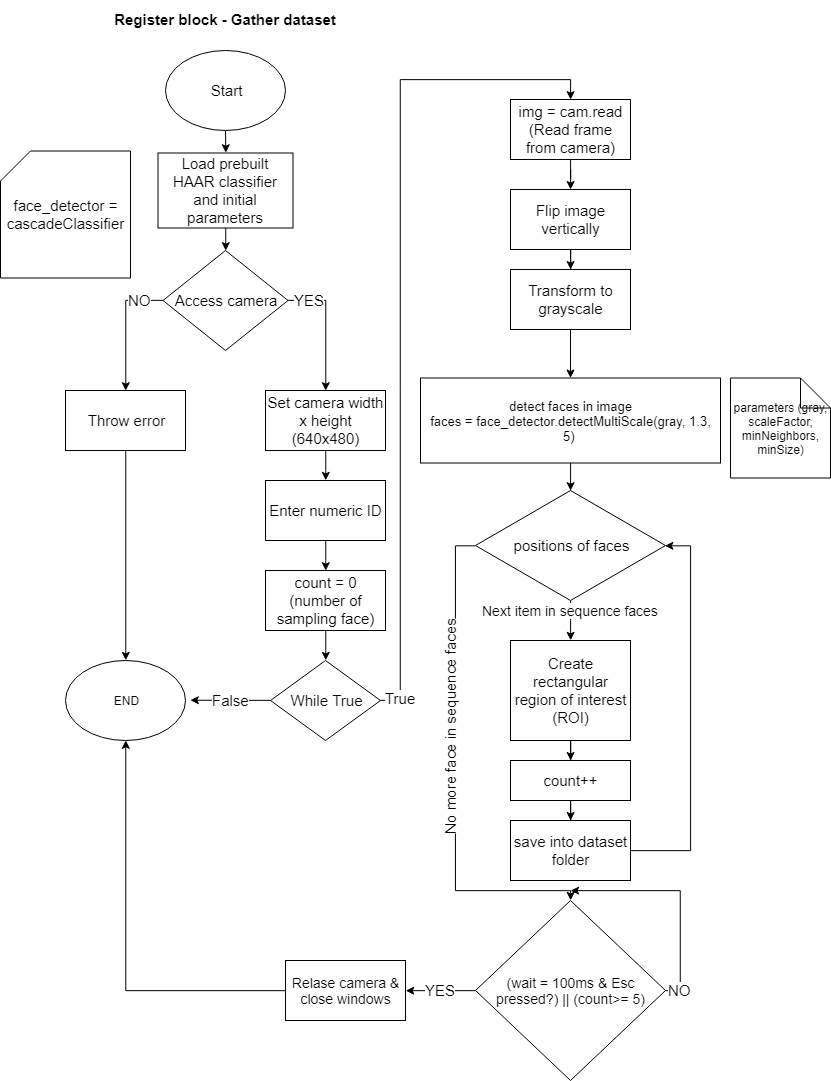
\includegraphics[scale=0.5]{images/dataset.png}
            \caption{Flowchart of Register step - Gathering dataset}
            \label{fig:dataset}
            \end{center}
        \end{figure}
        \begin{figure}[!ht]
            \begin{center}
            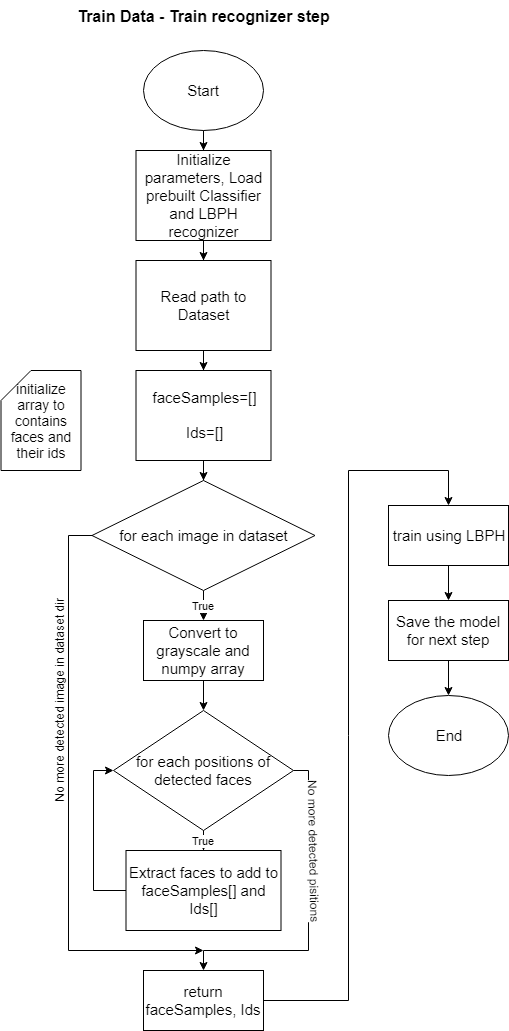
\includegraphics[scale=0.64]{images/train.png}
            \caption{Flowchart of Train data step - Training from dataset}
            \label{fig:train}
            \end{center}
        \end{figure}
        \begin{figure}[!ht]
            \begin{center}
            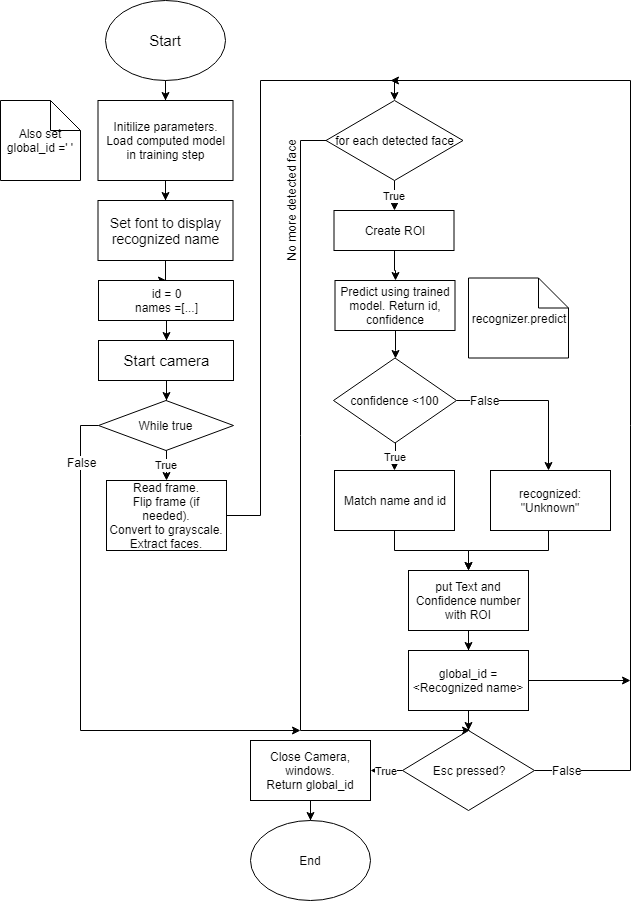
\includegraphics[scale=0.65]{images/recognize.png}
            \caption{Flowchart of Recognition step - Recognition from trained data}
            \label{fig:recognize}
            \end{center}
        \end{figure}
        
        
        
    


        






 
\chapter{Conclusion}
\section{Achievement}
\begin{itemize}
\item The model is successfully implemented with basic requirements of a conveniently house with physical buttons.
\item The control system is separately with the 220V AC line, which makes the system is a lots safer.
\item System can be extended with integrated communication ports.
\item The number of supported devices can be extended easily.
\item Devices in different rooms can be controlled with different buttons.
\item Successfully built a simple Web Server to control and monitor devices.
\item The Web Server is built with Responsive website design, which can be displayed correctly on different smart devices.
\item Integrated database to log data in order to monitor and maintain devices and may be used for further development.
\item Successfully implemented few scenarios to use.
\item Successfully implemented Outdoor Camera on embedded computer and prototype of Indoor Camera.
\item Implemented the system with MQTT protocol at few steps.
\end{itemize}
With this project, the author was able to improve and get to know more knowledge that he could never learn during the University time. Moreover, he also understands that he needs to keep studying to accumulate valuable experience which can be handy when entering the work space. However, the project still remain plenty of limitations as listed in following section. 

\section{Limitation}
\begin{itemize}
\item Limitation of used hardware.
\item Although the project is implemented with MQTT protocol for communication between the Internet block and the system, the delay is still a worth to consider.
\item The main communication methodology is not suitable for a small house.
\item Facial Recognition system is not as accurate as needed.
\end{itemize}

\section{Future Work}
\begin{itemize}
\item Replace RS-485 by (a) wireless communication methodology.
\item Optimize algorithm to reduce the delay between Slaves or System and Internet Block.
\item Integrate AI to make the house become truly smart.
\item Use collected data to build Markov Chain or Bayesian Models to predict if any device is forgot to turn On or Off at specified point of time, which helps the owner to use energy in more efficient way.
\item Improve the algorithm of Facial Recognition system for better performance.
\item Improve the aesthetics, stability and sustainable of the system included both hardware and software.
\end{itemize}


\end{document}